\documentclass[12pt]{article}

\usepackage[T1]{fontenc}
\usepackage{mathptmx}
\usepackage{graphicx}
\usepackage[hidelinks]{hyperref}
\usepackage{mathbbol,bm,amsmath,amsthm,amsfonts,amssymb}
\usepackage{mathtools}
\usepackage{booktabs}
\usepackage{fancyhdr}
\usepackage[mathscr]{euscript}
\usepackage[margin=0.5in]{geometry}
\usepackage{tikz}

\graphicspath{ {./images/}}

% Used for fancy bullet lists. Not really using it now
% \usepackage[shortlabels]{enumitem}
% \setlist[itemize]{label={$\bullet$}, topset=0.2ex, partopset=0pt, parsep=4pt, itemsep=0pt, leftmargin=4.5mm, labelsep=0.5ex}
% \setlist[enumerate]{align=left, listparindent=0pt}

\newcommand{\PP}{\mathscr{P}}
\newcommand{\R}{\mathbb{R}}
\newcommand{\N}{\mathbb{N}}
\newcommand{\Z}{\mathbb{Z}}
\renewcommand{\iff}{\;\leftrightarrow\;}
\newcommand{\floor}[1][x]{\lfloor #1\rfloor}
\newcommand{\ceil}[1][x]{\lceil #1\rceil}
\newcommand{\mat}[1][A]{\text{\textbf{#1}}}
\newcommand{\I}{\mathbb{1}}

\renewcommand{\thesubsection}{\arabic{subsection}}
\renewcommand{\thesubsubsection}{\alph{subsubsection}}

\title{\huge Exam preparation cheetzheet: \\ \textit{Stuff from}}

\author{\LARGE MNF130V2020}

\begin{document}

\maketitle

\bigskip

\newpage

\subsection{Chapter 1}
\smallskip
\textbf{Propositional logic}:. Logical $\wedge,\vee,\oplus$ are trivial. \\
\smallskip
\textbf{Conditional statements (implication)}: $p \rightarrow q$, if $p$ then $q \equiv p $ only if $q \equiv$ $p$ is a sufficient condition for $q$. \\
In other words, q is a necessary condition for p. $p \rightarrow q$ is false then $p$ is true and $q$ is false and otherwise true. \\
$\neg(p\rightarrow q)\equiv p \wedge (\neg q)$, $p \rightarrow q$ is equivalent to its contrapositive $\neg q \rightarrow \neg p$, but \textbf{not} to its \textbf{converse} $q \rightarrow p$ \textbf{or} its inverse $\neg p \rightarrow \neg q$. \\
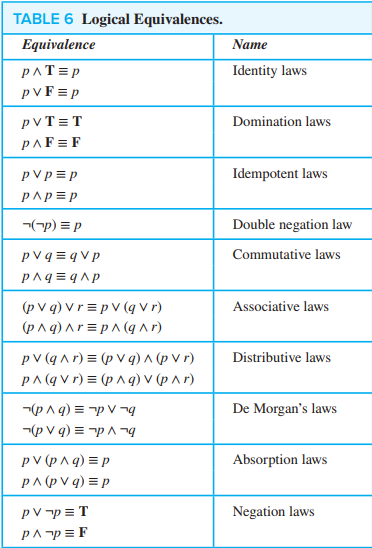
\includegraphics[scale=0.8]{logical_equivalences} \\
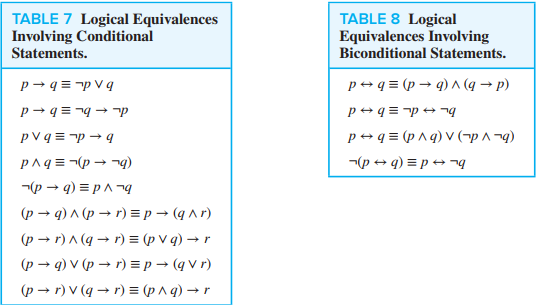
\includegraphics[scale=0.8]{logical_equivalences_conditional} \\
\smallskip
\textbf{Biconditional statements:} $ p \iff q$ or expanded to $(p \rightarrow q) \wedge (q \rightarrow p)$. \\
\smallskip{}
\textbf{De Morgan:} $\neg(p \vee q) \equiv (\neg p) \wedge (\neg q)\ ;\ \neg(p \wedge q) \equiv (\neg p ) \vee (\neg q) $
\smallskip
Propositional logic can be represented by gates, creating combinational circuits which can represent \textbf{any} logical expression. \\
\medskip
\textbf{Quantifiers:} \\
$
\forall x(P(x) \rightarrow Q(x)) \equiv
$
\textit{for all x, if P(x) then Q(x)} \\
$
\exists x(P(x) \wedge Q(x)) \equiv
$
\textit{there exists an x such that P(x) and Q(x)} \\

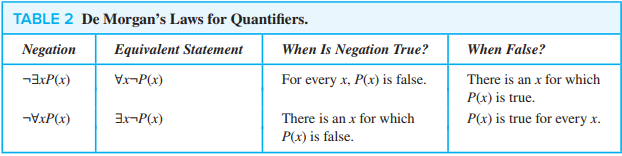
\includegraphics[scale=0.8]{de_morgan_quantifier_laws} \\
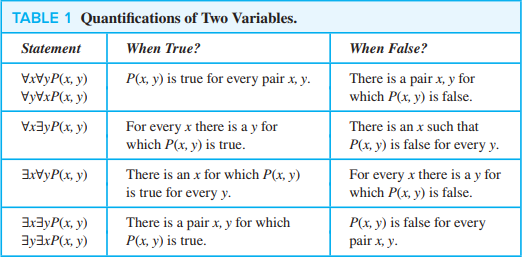
\includegraphics[scale=0.8]{multi_variable_quantifiers} \\
\textit{P(x),Q(x)} are propositional functions and there is always a \textbf{domain} or \textbf{universe of discourse}, either implicit or explicitly stated,over which the variable ranges. \\
\medskip
\textbf{Negations of quantified propositions:} $\neg \forall xP(x)\equiv \exists x\neg P(x); \neg \exists P(x) \equiv \forall x \neg P(x)$. \\
\medskip
\textbf{Theorem:} A proposition that can be proved; \textbf{lemma:} a simple theorem, commonly used as part of a greater picture to prove other theorems; \textbf{proof:} A demonstration that a proposition is true, \textbf{collorary:} A proposition that can be proved as a consequence of a theorem that has just been proved. A collorary can be seen as ``Side effects`` of the prooved theorem. \\
\medskip
A \textbf{valid} argument is an argument using correct rules of inference based on tautologies (something that will always give the \textbf{true} conclusion in \textbf{any} given scenario. I. E. a tautology is something that is always true for all possible combinations.) \\
An \textbf{invalid} argument can be referred to as a \textbf{fallacy}, such as affirming the conclusion, denying the hypothesis, begging the question or circular reasoning. They can lead to false conclusions. \\
\medskip
\textbf{Some rules of inference:} 
\begin{itemize}
\item $[ p \wedge (p \rightarrow q) ]$ Modus Ponens
\item $[ \neg q \wedge (p \rightarrow q)]$ Modus Tollens
\item $[(p \rightarrow q) \wedge (q \rightarrow r)] \rightarrow (p \rightarrow r)$ Hypothetical syllogism (Transitivity)
\item $[(p \vee q) \wedge (\neg p)] \rightarrow q$ Disjunctive syllogism
\item $\{P(a) \wedge \forall x [P(x) \rightarrow Q(x)]\} \rightarrow Q(a)$ Universal modus ponens
\item $\{\neg Q(a) \wedge \forall x[P(x) \rightarrow Q(x)]\} \rightarrow \neg P(a)$ Universal modus tollens
\item $(\forall x P(x)) \rightarrow P(c)$ Universal instantiation
\item $(P(c) arbitrary\ c) \rightarrow \forall xP(x)$ Universal generalization
\item $(\exists xP(x)) \rightarrow (P(c)\ for\ some\ c)$ Existential instantiation
\item $(P(c)\ for\ some\ element\ c) \rightarrow \exists x P(x)$ Existential generalization.
\end{itemize}
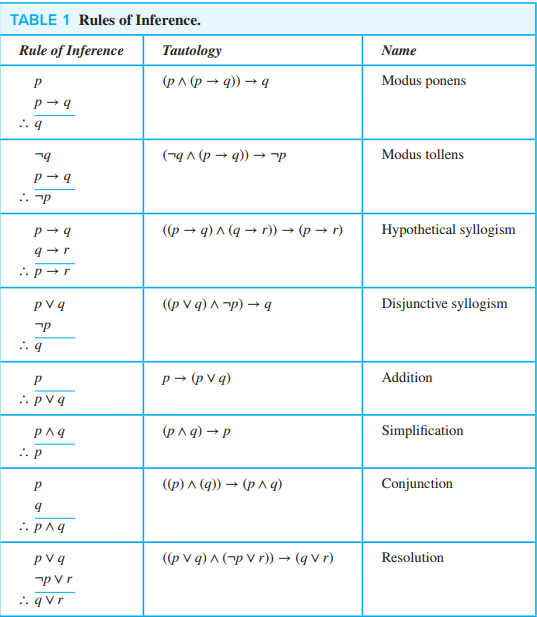
\includegraphics[scale=0.8]{rules_of_inference} \\
\newpage
\subsubsection{Proofs} 
\bigskip
\textbf{Trivial proof:} A proof that $p \rightarrow q$ just shows that $q$ is true witout using the hypothesis $p$. \\
\textbf{Vacuous proof:} A proof of $p \rightarrow q$ that just shows that the hypothesis $p$ is false. \\
\textbf{Direct proof:} A proof of $p \rightarrow q$ that shows that the assumption of the hypothesis $p$ implies the conclusion of $q$. \\
\textbf{Proof by contraposition:} A proof of $p \rightarrow q$ that shows that the assumption of the negation of the conclusion $q$ implies the negation of the hypothesis $p$ (in other words, proof of contrapositive).\\
\textbf{Proof by contradiction:} A proof of $p$ that shows that the assumption of the negation of $p$ leads to a contradiction. \\
\textbf{Proof by cases:} A proof of $(p_1 \vee p_2 \vee p_3 ... p_n) \rightarrow q$ that shows that each conditional statement $p_i \rightarrow q$ is true. Statements of the form $p \iff q$ require that both $p \rightarrow q$ and $q \rightarrow p$ be proved. It is sometimes necessary to give the two separate proof (usually a direct proof or a proof by contraposition); other times a string of equivalences can be constructed starting with $p$ and ending with $q : p \iff p_1 \iff p_2 ... \iff p_n \iff q$. \\
To give a \textbf{constructive proof} of $\exists x P(x)$ is to show how to find an element $x$ that makes $P(x)$ true. \textbf{Non-constructive existence proofs} are also possible, often using \textbf{proof by contradiction}. \\
One can \textbf{disprove} a universally quantified proposition $\forall x P(x)$ simply by giving a \textbf{counter example}, i.e. an object $x$ such that $P(x)$ is \textbf{false}. One can, however, not proove it with such an example. \\
\medskip
\textbf{Fermat's last theorem:} There are no positive integer solutions of $x^n + y^n = z^n\ if\ n > 2$. \\
An integer is \textbf{even} if it can be written as $2k$ for some integer $k$; an integer is \textbf{odd} if it can be written as $2k + 1$ for some integer $k$. Every number is even or odd but not both. A number is \textbf{rational}, if it can be written as $p/q$ with $p$ being an integer and $q$ strictly a non-zero integer. \\
\newpage
\subsection{Chapter 2}
\subsubsection{Sets}
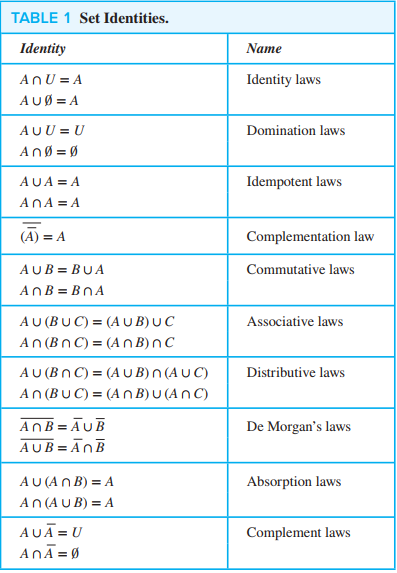
\includegraphics[scale=0.8]{set_identities} \\
\textbf{Empty set:} A set with no elements, commonly denoted as $\emptyset$. Do not confuse this with the set only containing the empty set. The difference is that the empty itself is empty, whereas the set containing the empty set has a single element. \\
\textbf{Subset:} $A \subseteq B \equiv \forall x(x \in A \rightarrow x \in B)$, whereas a proper subset is $ A \subset B \equiv (A \subseteq B) \wedge (A \neq B)$, in other words, $B$ has at least one element different from the set $A$. \\
\textbf{Equality of sets:} $A = B \equiv (A \subseteq B \wedge B \subseteq A) \equiv \forall x(x \in A \leftrightarrow x \in B)$. \\
\textbf{Power set:} $\PP(A) = \{B | B \subseteq A \}$, the set of all subsets of $A$. A set with $n$ elements has $2^n$ subsets. \\
\textbf{Cardinality:} $|S|$, the number of elements in $S$. \\
Some specific sets in regards to cardinality: $\R$ is the set of real numbers, represented by either finite or infinite decimals; \\
$\N$ is the set of all natural numbers (eg. $\{0,1,2,3,4,5...\}$), $\Z$ is the set of integers $\{... -2, -1, 0, 1, 2, ...\}$ and can also be denoted with only the positive or negative subset. $\mathbb{Q}$ is the set of rational numbers, where $\{ p / q | p, q \in \Z \wedge q \neq 0 \}$, $\mathbb{Q}^+$ is the set of positive rational numbers and a subset of $\mathbb{Q}$. \\
\textbf{Set operations:} $A \times B = \{ (a,b) | a \in A \wedge b \in B\}$ (\textbf{Cartesian Product}); $\overline{A}$ is the set of elements in the universe which are \textbf{not} in $A$ (\textbf{complement}); $A \cap B = \{ x | x \in A \wedge x \in B\}$ (\textbf{intersection}); $A \cup B = \{ x | x \in A \vee x \in B\}$ (\textbf{union}); \\
$A - B = A \cap \overline{B}$ (\textbf{difference}); $A \oplus B = (A - B) \cup (B - A)$, (\textbf{symmetric difference/xor}) \\
\textbf{Inclusion-exclusion (simple case):} $|A \cup B| = |A| + |B| - |A \cap B|$\\
\textbf{De Morgan's laws for sets:} $\overline{A \cap B} = \overline{A} \cup \overline{B}$; $\overline{A \cup B} = \overline{A} \cap \overline{B}$ \\
A \textbf{function} f from $A$ (\textbf{the domain}) to $B$ (\textbf{the co-domain}) is an assignment of a unique element of $B$ to each element of $A$. Write $f: A \rightarrow B$. Write $f(a) = b$ if $b$ is assigned to $a$. \textbf{Range} of $f$ is $\{ f(a) | a \in A\}$; $f$ is \textbf{onto/surjective} $\equiv$ range $(f)$ = $B$; $f$ is \textbf{one-to-one/injective} $\equiv$ $\forall a_1 \forall a_2 [f(a_1) = f(a_2) \rightarrow a_1 = a_2]$ \\
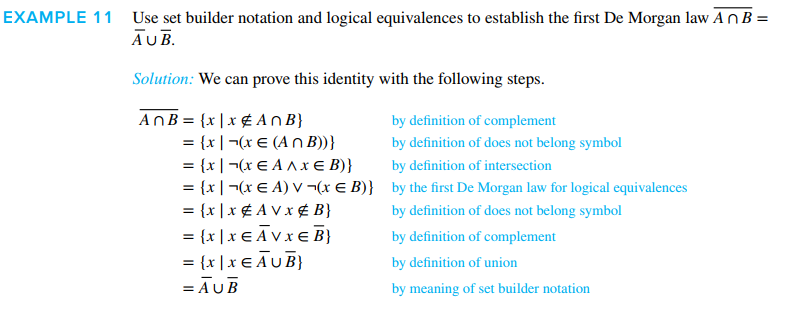
\includegraphics[scale=0.8]{set_de_morgan} \\
If $f$ is one-to-one \textbf{and} onto, it is \textbf{bijective} and the \textbf{inverse} function $f^{-1} : B \rightarrow A$ is defined by $f^{-1}(y) = x \equiv f(x) = y$. \\
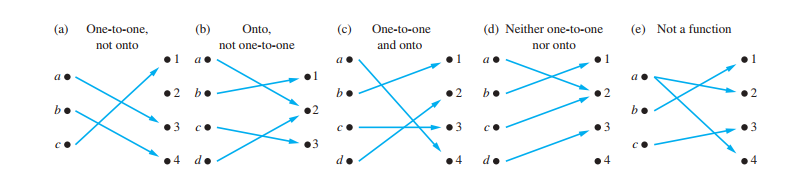
\includegraphics[scale=0.8]{function_correspondance}\\
If $f : B \rightarrow C$ and $g : A \rightarrow B$, then the \textbf{composition} $f \circ g$ is the function from $A$ to $C$ defined by $f \circ g(x) = f(g(x))$. \\
\textbf{Rounding functions:} $\floor{}$ is the largest integer less than or equal to x \textbf{floor function}; $\ceil{}$ is the smallest integer greater than or equal to $x$ \textbf{the ceiling function}. \\
\textbf{Summation notation:}

$$
\sum_{n=1}^{n} a_i = a_1 + a_2 + a_3 + ... + a_n
$$
\textbf{Sum of first $n$ positive integers:} 
$$
\sum_{j=1}^{n} j = 1 + 2 + ... + n = \frac{n(n +1)}{2}
$$
\textbf{Sum of squares of first $n$ positive integers:}
$$
\sum_{j=1}^{n} j^2 = 1^2 + 2^2 + ... + n^2 = \frac{n(n +1)(2n+1)}{6}
$$
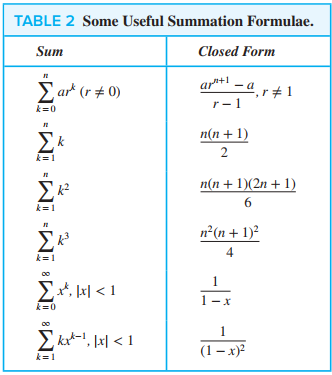
\includegraphics[scale=0.8]{summation_formulae} \\
\textbf{Sum of geometric progression:}
\textit{(I don't think we did this in the course)}\\ 
\newpage
Two sets are said to have the \textbf{same cardinality} if there is a \textbf{bijection} between them. We can say that $|A| \leq |B|$ if there is a one-to-one function from $A$ to $B$. \\
A set is $countable$ if it is finite or there is a \textbf{bijection} from the positive integers to the set. \textbf{In other words}, if the elements of the set can be listed (e.g. $a_1, a_2, ...$). Sets of the latter type are called $countably infinite$ and the \textbf{cardinality of these sets are denoted with $\aleph_0$ }. The empty set, the integers and the rational numbers \textbf{are countable}. The union of a countable number of countable sets is countable. \\
\textbf{Schroder-Bernstein theorem:} If $|A| \leq |B|$ and $|B| \leq |A|$ then it must be that $|A| = |B|$. This can be explained as if there is a one-to-one function from A to B and a one-to-one function from B to A, then there is a one-to-one and onto function from A to B. \\
\textbf{Matrix Multiplication:} The $(i,j)^{th}$ entry of \textbf{AB} is $\sum_{t=1}^k a_{it}b_{tj}$ for $1 \leq i \leq m$ and $1 \leq j \leq n$, where \textbf{A} is an $m \times k$ matrix and \textbf{B} is a $k \times n$ matrix. \\
\textbf{Identity matrix $I_n$} with 1's on the main diagonal and 0's elsewhere is the multiplicative identity. \\
Cardinality arguments can be used to show that some functions are \textbf{uncomputable}. \\
Matrix addition (+), Boolean meet ($\wedge$) and join ($\vee$) are done entry-wise; Boolean matrix product ($\odot$) is like matrix multiplication using boolean operators. \\
\textbf{Transpose:} \textbf{A}$^t$ is the matrix whose $(i,j)^{th}$ entry is $a_{ij}$ (the $(j,i)^{th}$ entry of \textbf{A}); \\
\textbf{A} is \textbf{symmetric} if \textbf{$A^t=A$};
\newpage
\subsection{Chapter 3}
\textbf{Algorithm} are commonly expressed in \textbf{pseudo-code} when not directly implemented in a domain specific area. \\
\textbf{Keywords for algorithms:} \{input, output, definiteness, correctness, finiteness, effectiveness, generality\}. \\
\textbf{Greedy algorithms:} Will examine and pick the best choice at a given step. Not always the best. \\
\textbf{Brute forcing:} Specifically in discrete mathematics, this referres to examining the entire space of solutions and then determine the best one (very inefficient, sometimes necessary). Not explained in this course: \textbf{dynamic programming, probabilistic algorithms, divide-and-conquer}. \\
\textbf{Halting problem:} The unsolvable computing problem whether a program will halt given input. (Alan Turing for reference...) \\
\textbf{Big-O:} Half of inf102 is just this: \\
$f(x) = O(g(x))$ means $\exists C\exists k \forall x(x > k \rightarrow |f(x)| \leq C|g(x)|)$. Big-O of a sum is the largest (fastest growing) of the functions in the sum. Big-O of a product is the product of the big-O's of the factors. If $f$ is $O(g)$, the $g$ is $\Omega (f)$ "big-omega". If $f$ is both big-O and big-Omega of $g$, then $f$ is $\theta (g)$ "big-theta". \\
\textbf{Little-O:} We say that $f(x)$ is $o(g(x))$ if $\lim_{x\rightarrow \infty}f(x)/g(x) =0$.\\
\textbf{Powers grow faster than logs:} $(\log n)^c$ is $O(x^d)$ but not the other way around, where $c$ and $d$ are positive numbers. \\
If $f_1(x)$ is $O(g_1 (x))$ and $f_2(x)$ is $O(g_2(x))$, then $(f_1+f_2)(x)$ is $O(\max (g_1(x),g_2(x)))$ and $(f_1f_2)(x)$ is $O(g_1(x)g_2(x))$. \\
$\log n!$ is $O(n \log n)$. \\
\textbf{Time complexity:} Binary search = $O(\log n)$ (cut half of possibilites at each step), linear search $O(n)$ (all input is examined exactly once), both have \textbf{space complexity (in terms of computer memory) O(1)} without taking the input into account. Bubble sort and insertion sort have $O(n^2)$. \\
Matrix multiplication has standard algorithm time complexity of $O(m_1m_2m_3)$ if the matrices have dimensions $m_1 \times m_2$ and $m_2 \times m_3$. \\
Efficient algorithms can reduce the complexity of multiplying two $n \times x$ matrices from $O(n^3)$ to $O(n^{\sqrt{7}})$
Important complexity classes include polynomials $n^b$, exponential ($b^n$ for $b > 1$) and factorial ($n!$). \\
A problem that can be solved by an algorithm with polynomial worst-case time complexity is called \textbf{tractable}; otherwise \textbf{intractable}. \\
\textbf{P=NP problem:} The class \textbf{P} is the class of tractable problems. The class \textbf{NP} consists of the problems for which it is possible to check solutions (\textbf{not FIND solutions}) in polynomial time. This means that \textbf{$P \subseteq NP$} yet the \textbf{P=NP} problem is unsolved because it has not been shown whether \textbf{P=NP}.
\newpage
\subsection{Chapter 4}
\textbf{Divisibility:} $a | b$ means $a \neq 0 \wedge \exists c(a\cdot c=b)$ ($a$ is a \textbf{divisor} or \textbf{factor} of $b$ such that $b$ is a multiple of $a$). \\
\textbf{Base $b$ representiations:} ($a_{n-1}a_{n-2}...a_2a_1a_0$)$_b = a_{n-1}b^{n-1}+...+a_2b^2+a_1b+a_0$.\\
To convert from base 10 to base $b$, continually divide by $b$ and record remainders as $a_0,a_1,a_2,...$ ($b=8$ is \textbf{octal}, $b=16$ is \textbf{hexadecimal}, using A-F for 10-15). Convert from binary to octal by grouping bits by \textbf{threes}, from the right, to hexadecimal by grouping by fours; because $2^3=8$ and $2^4=16$. \\
\textbf{Addition:} of two \textbf{binary numerals} each of $n$ bits (($a_{n-1}a_{n-2}...a_2a_1a_0$)$_2$) requires $O(n)$ bit operations.\\
\textbf{Multiplication:} requires $O(n^2)$ bit operations if done naively, $O(n^{1.585})$ steps by more sophisticated algorithms. \\
\textbf{Division "algorithm":}
$$
\forall a \forall d > 0 \exists q \exists r (a = dq + r \wedge 0 \leq r < d)
$$
where $q$ is the quotient and $r$ is the remainder; we write $a$ \textbf{mod} $d$ for the remainder. \\
\textbf{Example of the division "algorithm":}
$$
-18 = 5 \cdot (-4) + 2 \rightarrow -15\ \textbf{mod}\ 5 = 2
$$\\
\textbf{Congruent modulo $m$:} $a \equiv b (\ mod\  m) \iff m | a - b \iff a\ mod\ m = b\ mod\ m$ \\
One can do arithmetic in $\Z_m = \{ 0,1,...,m-1\}$ by working modulo $m$. There are fast algorithms for computing $b^n\ mod\ m$, based on successive squaring. \\
Integer $n > 1$ is said to be \textbf{prime} $\iff$ its only factors are 1 and itself; otherwise it is referred to as a \textbf{composite}. \\
There are infinitely many \textbf{primes}, but it is not known whether there are infinitely many twin primes (\textbf{primes that differ by 2}), or whether every even positive integer greater than 2 is the sum of two primes (\textbf{Goldbach's conjecture}) or whether there are infinitely many \textbf{Mersenne primes $\rightarrow$ primes of the form $2^p -1$}. \\
\textbf{Naive test for primeness and test for prime factorization:} To find prime factorization of $n$, successively divide it by all primes less than $\sqrt{n}$; if none is found, then \textbf{n is prime}. If a prime factor $p$ is found, then continue the process to find the prime factorization of the remaining factor, namely $n/p$; this time the trial divisions can start with $p$. Continue until a prime factor remains. \\
\textbf{Prime number theorem} states that there are approximately $n/\ln(n)$ primes less than or equal to $n$. \\
\textbf{Fundamental theorem of arithmetic:} Every integer greater than 1 can be written as a product of one or more primes, and the product is unique except for the order of the factors. (A proof based on fact that if a prime divides a product of integers, then it divides at least one of those integers.) \\
\textbf{Euclidean algorithm for greatest common divisor}: $gcd(x,y) = gcd(y,x\ \textbf{mod}\ y)$ if $y \neq 0$; $gcd(x,0)=x$. \\
Using extended Euclidean algorithm or working backwards, one can find \textbf{Bezout coefficients} and write $gcd(a,b) = sa+tb$. \\
Two integers are \textbf{relatively prime} if their greatest common divisor (gcd) is 1. The integers $a_1,a_2,...,a_n$ are \textbf{pairwise relatively prime} $\iff gcd(a_i,a_j) = 1$ whenever $1 \leq i < j \leq n$. \\
\textbf{Chinese reminder theorem:} If $m_1,m_2,...m_n$ are pairwise relatively prime, then the system $\forall i(x\equiv a_i (\ mod\ m_i))$ has unique solution modulo $m_1m_2...m_n$. An example of application of this: Handling very large integers on a computer. \\
\textbf{Fermat's little theorem:} $a^{p-1} \equiv 1 (\ mod\ p)$ if $p$ prime and does not divide $a$. The converse is not true; for example $2^{340} \equiv 1(\ mod\ 341)$ so $341(=11\cdot 31)$ is referred to as a \textbf{pseudo prime}; \\
If $a$ and $b$ are positive integers, then there exist integers $s$ and $t$ such that $as+bt = gcd(a,b)$ \textbf{linear combination}. \\
This theorem allows one to compute the \textbf{multiplicative inverse} $\overline{a}$ of $a\ modulo\ b$ (i.e $\overline{a}a \equiv 1 (\ mod\ b))$ as long as $a$ and $b$ are relatively prime, which enables one to solve \textbf{linear congruences} $ax \equiv c (\ mod\ b)$. \\
\textbf{A primitive root} modulo a prime $p$ is an integer $r$ in $\Z_p$ such that every nonzero element of $\Z_p$ is a power of $r$. \\
\textbf{Discrete logarithms:} $\log_r a = e$ modulo $p$ if $r^e$ \textbf{mod} $p = a$ and $1 \leq e \leq p -1$  \\
A common \textbf{hashing function:} $h(k) = k\ \textbf{mod}\ m$, where $k$ is the key. \\
\textbf{Check digits} for error-correcting codes like UPCs, involve modular arithmetic (??????????) \\
\textbf{Pseudorandom numbers:} can be generated by the \textbf{linear congruential method:} $x_{n+1} = (ax_n +c)\ \textbf{mod}\ m$, where $x_0$ is arbitrarily chosen \textbf{seed}. Then $\{x_n/m\}$ will be rather randomly distributed numbers between 0 and 1. \\
\textbf{Shift cipher:} $f(p) = (p + k)\ \textbf{mod}\ 26 [A \iff 0, B \iff 1,...]$. Caeser cipher used $k=3$. \\
\textbf{Affine cipher:} Uses $f(p) = (ap+b)\ \textbf{mod}\ 26$ with $gcd(a,26)=1$. \\
\textbf{RSA public key encryption system:} An integer $M$ representing the plaintext is translated into an integer $C$ representing the ciphertext using the function $C = M^e\ \textbf{mod}\ b$, where $n$ is a public numbers that is the product of two large (100-digit or so) primes and $e$ is a public number \textit{relatively} prime to $(p-1)(q-1)$; the primes $p$ and $q$ are kept secret. Decryption is accomplished via $M=C^d\ \textbf{mod}\ n$, where $d$ is an inverse of $e$ modulo $(p-1)(q-1)$. It is infeasible to compute $d$ without knowing $p$ and $q$, which are infeasible to compute from $n$. \\
Similar methods can be used for \textbf{key exchange protocols}, \textbf{digital signatures}, \textbf{signing stuff in general}. \\
\newpage
\subsection{Chapter 5}
\textbf{The well-ordering property:} Every non-empty set of nonnegative integers has a "least element". \\
\textbf{The principle of mathematical induction:} Let $P(n)$ be a propositional function in which the domain (the universe of discourse) is the set of positive integers. Then if one can show that $P(1)$ is true (through \textbf{Base case/Base step}) and that for every positive integer $k$, the conditional statement $P(k) \rightarrow P(k+1)$ is true \textbf{(inductive step)}, then one has proved that $\forall n P(n)$. The hypothesis $P(k)$ in a proof of the inductive step is called the \textbf{inductive hypothesis}. \\
More generally, the indcution can start at any integer, and there could potentially be several base cases. \\
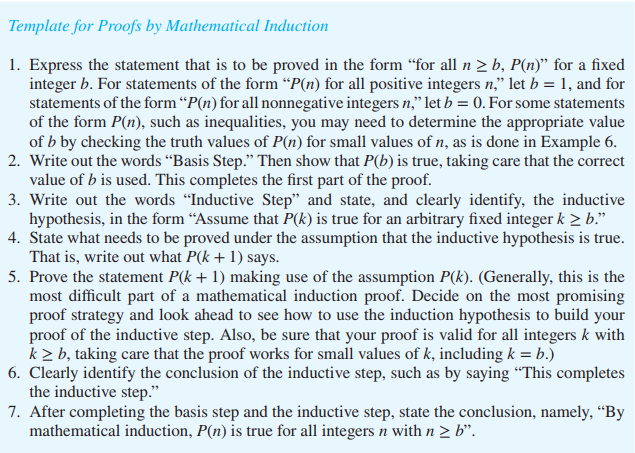
\includegraphics{induction_template} \\
\textbf{Strong induction:} Let $P(n)$ be a propositional function in which the domain (again, \textbf{universe of discourse}) is the set of positive integers. Then if one can show that $P(1)$ is true, and that for every positive integer $k$ the conditional statement $[P(1) \wedge P(2) \wedge ... \wedge P(k)] \rightarrow P(k + 1)$ is true \textbf{(inductive step)}, then one has proved $\forall n P(n)$. The hypothesis $\forall j \leq k P(j)$ in a proof of the inductive step is called the (\textbf{(strong) inductive hypothesis}). Again, the induction can start at any integer, and there can be several base cases. \\
\textbf{Inductive/Recursive definitions (functions):} Is a definition of a function $f$ with the set of nonnegative integers as its domain: Specification of $f(0)$, together with, for each $n > 0$, a rule for finding $f(n)$ from values of $f(k)$ for $k < n$. \\
\textbf{Example:} $0! = 1$ and $(n + 1)! = (n + 1) \cdot n!$ \textbf{(factorial function)} \\
\medskip
\textbf{Inductive/Recusive definitions (sets):} Definition of a set $S$: A rule specifying one or more particular elements of $S$, together with a rule for obtaining more elements of $S$ from those already in it. It is understood that $S$ consists precisely of those elements that can be obtained by applying these two rules. \\
\textbf{Structural induction:} can be used to prove facts about recursively defined objects. \\
\textbf{Fibonacci numbers}: $f_0,f_1,f_2,...: f_0 = 0, f_1 = 1,f_n = f_{n-1} + f_{n-2}$ for all $ n \geq 2$. \\
\textbf{Lame's theorem:} The number of divisions used by the Euclidean algorithm to find $gcd(a,b)$ is $O(\log b)$. \\
An algorithm is \textbf{recursive} if it solves a problem by reducing it to an instance of the same problem with smaller input. It is \textbf{iterative} if it is based on the repeated use of operations in a loop. \\
There is an efficient recursive algorithm for computing \textbf{modular powers ($b^n$ mod $m$)}, based on computing $b^{[\frac{n}{2}]}$ \textbf{mod} $m$. \\
\textbf{Merge sort:} is an efficient recursive algorithm for sorting a list: break the list into two parts, recursively sort each half, and then merge them together in order. It has $O(n\log n)$ time complexity in \textbf{all} cases. \\
A program segment $S$ is \textbf{partially correct} with respect to \textbf{initial assertion} $p$ and \textbf{final assertion} $q$, written $p\{S\}q$, if whenever $p$ is true for the input values of $S$ and $S$ terminates, $q$ is true for the output values of $S$. \\
A \textbf{loop invariant} for \textbf{while} $condition\ S$ is an assertion $p$ that remains true each time $S$ is executed in the loop; \\
i.e. $(p\wedge\ condition)\{S\}p$. If $p$ is true before the program segment is executed, then $p$ and $\neg condition$ are true after it terminates (if it terminates at all). In symbols, $p\{\textbf{while}\ condition\ S\}(\neg condition\ \wedge p)$.
\newpage
\subsection{Chapter 6}
\textbf{Sum rule:} Given $t$ mutually exclusive tasks, if task $i$ can be done in $n_i$ ways, then the number of ways to do exactly one of the tasks is $n_1 + n_2 + ... + n_t$.\\
\textbf{Size of union of \underline{disjoint} sets:} $|A_1 \cup A_2 \cup ... \cup A_n | = |A_1| + |A_2| + ... + |A_n|$. ?? Duplicates ??\\
\textbf{Two-set case of inclusion-exclusion:} $|A \cup B| = |A| + |B| - |A \cap B|$.
\textbf{Product rule:} If a task consists of successively performing $t$ tasks, and if task $i$ can be done in $n_i$ ways (after previous tasks have been completed), then the number of ways to do the task is $n_1 \cdot n_2 ... n_t$. \\
A set with $n$ elements has $2^n$ subsets (equivalently, there are $2^n$ bit strings of length $n$). \\
\textbf{Tree diagrams:} Can be used to organize counting problems. \\
\textbf{Pigeonhole principle:} If more than $k$ objects are placed in $k$ boxes, then some box will have more than 1 object.\\
\textbf{Generalized version of the pigeonhole principle:} If $N$ objects are placed in $k$ boxes, then some box will have at least $[N/k]$ objects. \\
\textbf{Ramsey number:} $R(m,n)$ is the smallest number of people there must be at a party so that there exist either $m$ mutual friends or $n$ mutual enemies (assuming each pair of people are either friends or enemies). $R(3,3) = 6$. \\
\textbf{r-permutation} of set with $n$ objects, \textit{ordered} arrangement of $r$ of the objects from the set (no repetitions allowed); there are $P(n,r) = n!/(n-r)!$ such permutations.
\textbf{r-combination} of set with $n$ objects, \textit{unordered} selection (i.e subset) of $r$ of the objects from the set (no repetitions allowed); there are $C(n,r) = n!/[r!(n-r)!]$ such combinations. Alternative notation is $\begin{pmatrix} n \\ r\end{pmatrix}$, also called the binomial coefficient. \\
\textbf{Pascal's identity:} \textit{not in curriculum}. \\
\textbf{Combinatorial identities:} \textit{not in curriculum}. \\
Number of \textbf{r-permutations} of an $n$-set \textbf{with repetitions allowed} is $n^r$; number of \textbf{r-combinations} of an $n$-set \textbf{with repetitions} allowed is $C(n +r - 1,r)$. This latter value is the same as the \textbf{number of solutions in nonnegative integers} to $x_1 + x_2 + ... + x_n =r $. \\
\newpage
\subsection{Chapter 7} 
If all outcomes are equally likely in a \textbf{sample space} $S$ with $n$ outcomes, then the \textbf{probability of an event $E$} is $p(E) =|E|/n$; more generally, if $p(s_i)$ is probability of $i^{th}$ outcome $s_i$, then $p(E) = \sum_{s_i \in E} p(s_i)$. \\
\textbf{Probability distributions:} satisfy these conditions: $0 \leq p(s) \leq 1$ for each $s \in S$ and $\sum_{s \in S} P(s) = 1$. \\
For \textbf{complementary event}, $p(\overline{E}) = 1 - p(E)$; for \textbf{union} of two events (either one or both happen), $p(E\cup F) = p(E) + p(F) - p(E \cap F)$; for \textbf{independent events}, $p(E \cap F) = p(E)p(F)$. \\
The \textbf{conditional probability} of $E$ given $F$ (probability that $E$ will happen after it is known that $F$ happened) is $p(E|F) = p (E \cap F)/p(F)$. \\
\textbf{Bernoulli trials:} If only two outcomes are \textbf{success} and \textbf{failure}, with $p(success) = p$ and $p(failure) = q = 1 - p$, then the \textbf{binomial distribution} applies, with probability of exactly $k$ success in $n$ trials being $b(k;n,p) = C(n,k)p^kq^{n-k}$. \\
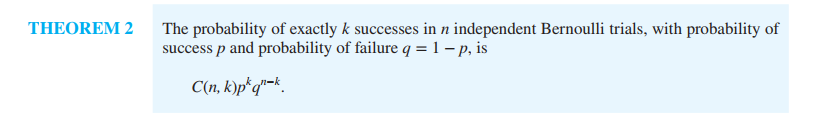
\includegraphics[scale=0.8]{bernoulli}\\
\textbf{Bayes Theorem:} \textit{Dont think this was in the curriculum}.\\
\newpage
\subsection{Chapter 9 (Chapter 8 not in curriculum)}
\textbf{(Binary) Relations:} A binary relation $R$ from $A$ to $B$: subset of the \textbf{cartesian} set $A \times B$. Write $aRb$ for $(a,b) \in R$; relation \textbf{on} $A$ is relation from $A$ to $A$; graph of a function from $A$ to $B$ is a relation such that $\forall a \in A \exists $ exactly one pair $(a,b)$ in the relation. \\
Relation $R$ on a set $A$ is \textbf{reflexive} if $aRa$ for all $a \in A$.\\
\textbf{Irreflexive} if $aRa$ for no $a \in A$. \\
\textbf{Symmetric} if $aRb$ implies $bRa$ for all $a,b \in A$. \\
\textbf{Asymmetric} if $aRb$ implies that $b$ is not related to $a$, for all $a,b \in A$. \\
\textbf{Antisymmetric} if $aRb \wedge bRa$ implies $a = b$ for all $(a,b) \in A$. \\
\textbf{Transitive} if $aRb \wedge bRc$ implies $aRc$ for all $a,b,c \in A$. \\
\textbf{Inverse} relation to $R$ is given by  $bR^{-1}a \iff aRB$. \\
If $R$ is a relation from $A$ to $B$ and $S$ is a relation from $B$ to $C$, then the \textbf{composite} is the relation $S \circ R$ from $A$ to $C$ in which $a$ is related to $c \iff$ there exists a $b \in B$ such that $aRb$ and $bSc$. $R^n = R \circ R \circ ... \circ R$. \\
\textbf{N-ary relations:} on domains $A_1,A_2,...,A_n$ is a subset of $A_1 \times A_2 \times ... \times A_n$; databases using the relational data model are just sets of \textbf{n-ary} relations in which each $n$-tuple is called a \textbf{record} made up of \textbf{fields} ($n$ is the \textbf{degree}). \\
\textbf{A relation as matrix representation:} A relation $R$ on $A = \{ a_1,a_2,...,a_n\}$ can be represented by an $n \times x$ matrix $M_R$ whose $(i,j)^{th}$ entry is 1 if $a_iRa_j$ and is 0 otherwise. Reflexivity, symmetry, antisymmetry, transitivity can easily be read off the matrix. Boolean products of the matrices give the matrix for the composite ($M_{S \circ R} = M_R \odot M_S$). \\
A domain is a \textbf{primary key} if the corresponding field uniquely determines the record. \\
\textbf{Equivalence classes:} A relation $R$ of set $A$ is an \textbf{equivalence relation} if $R$ is reflexive, symmetric and transitive. Usually, equivalence relations can be recognized by their definitions being of the form "two elements are related $\iff$ they have the same [something]". \\
For each $a \in A$ the set of elements in $A$ related to (i.e \textbf{equivalent to}) $a$ is the \textbf{equivalence class} of $a$, denoted [$a$]. \\
\textbf{Canonical example:} Congruence modulo $m$ with equivalence. \\
The set of equivalence classes partitions $A$ into pairwise disjoint nonempty sets; conversely, every partition of $A$ induces an equivalence relation by declaring two elements to be related if they are in the same set of the partition. 
\newpage
\subsection{Chapter 10} 
\textbf{Simple graph:} $G =(V,E)$ consists of a nonempty set of \textbf{vertices (singularis: vertex)}, and a set of unordered pairs of distinct vertices called \textbf{edges}. \\
\textbf{A multigraph:} allows more than one \textbf{edge} joining the same pair of vertices (called \textbf{multiple edges or parallel edges}); $E$ is just a set with an endpoint function $f$ taking each edge $e$ to its two $distinct$ endpoints. \\
\textbf{A pseudograph:} A pseudograph is like a multigraph but enpoints $f(e)$ need not be distinct, allowing \textbf{loops}. \\
\textbf{A directed} graph is also called a \textbf{digraph}, it is like a simple graph except that the edges are directed (they have an arrow/ a direction attached to them) (each $e$ is an $ordered pair$, and loops are allowed). \\
\textbf{A directed multigraph} is just like a multihgraph with parallel edges allowed, except that edges are directed (loops are allowed). \\
Given a directed graph, we can ignore order and look at the \textbf{underlying undirected graph.} \\
\textbf{Graphs can be used to model relationships:} herein examples such as: \textbf{acquaintances, food webs, telephone calls, networks, roads, internet, tournaments, organizations}. \\
\textbf{Vertices joined by an edge} are \textbf{adjacent} and the edge is \textbf{incident} to them. \\
\textbf{A degree of a vertex (deg(v))} is the number of incident edges, with loops counted double. An \textbf{isolated vertex} has degree 0, a \textbf{pendant vertex} has degree 1. \\
\textbf{A regular graph} has all degrees equal. \\
In a \textbf{digraph}, $deg(v^-f)$ is the number of edges leading into $v$ (\textbf{in-degree; v is terminal vertex}), and $deg(v^+)$ is number of edges leading out of $v$ (\textbf{out-degree; v is initial vertex}). \\
\textbf{Bipartite graph:} vertex set can be partitioned into two nonempty sets with no edges joining vertices in same set. \\
\textbf{The complete graph:} $K_n$ has $n$ verttices and an edge joining every pair $(n(n-1)/2))$ edges in all. \\
\textbf{Complete bipartite graph} $K_{m,n}$ has $m+n$ vertices in parts of sizes $m$ and $n$ and an edge joining every pair of vertices in different parts ($mn$ edges in all). The \textbf{cycle} $C_n$ has $n$ vertices and $n$ edges, joined in a circle. \textbf{The wheel} $W_n$ is $C_n$ with one more vertex joined to these $n$ vertices. The \textbf{cube} $Q_n$ has all $n$-bit binary strings for vertices, with an edge between every pair of vertices differing in only one bit position. \\
\textbf{(V,E) is subgraph} of $(W,F)$ if $V \subseteq W$ and $E \subseteq F$. \\
\textbf{Union} of two simple graphs is formed by taking union of corresponding vertex sets and corresponding edge sets. \\
\textbf{Graphs can be represented by an adjancancy matrix:} $m$ in position $(i,j)$ denotes $m$ parallel edges from $i$ to $j$. \textbf{Adjacency lists, incidence matrix} (1 is position $(i,j)$ says that vertex $i$ is incident to edge $j$). \\
\textbf{Graphs are isomorphic} if there is a bijection between vertex sets that preserves all adjacencies and nonadjacencies. To show graphs are \textbf{not} isomorphic, find \textbf{invariant} on which they differ (e.g. degree sequence, existence of cycles). \\
\textbf{A path} of length $n$ from $u$ to $v$ is a sequence of $n$ edges leading successively from $u$ to $v$; is a \textbf{circuit} if $n > 0$ and $ u = v$, is \textbf{simple} if no edge occurs more than once. \\
\textbf{A graph is connected} if every pair of vertices is joined by a path. A digraph is \textbf{strongly connected} if every pair of vertices is joined by a path in each direction, \textbf{weakly connected} if underlying undirected graph is connected. \\
\textbf{Components} are maximal connected subgraphs.\\
\textbf{Removal of cut edge (bridge)} or \textbf{cut vertex (articulation point)} creates more components.  

\end{document}